\documentclass[11pt,a4paper]{article}

% ---------------------------------------------------------------------------
% AI651 Assignment 2 -- Question 1: River Forecasting Proposal
% Compile with pdfLaTeX (Overleaf default).
% ---------------------------------------------------------------------------
\usepackage[margin=1.8cm]{geometry}
\usepackage[T1]{fontenc}
\usepackage{lmodern}
\usepackage{amsmath,amssymb}
\usepackage{bm}
\usepackage{array}
\usepackage{booktabs}
\usepackage{tabularx}
\usepackage{enumitem}
\usepackage{xcolor}
\usepackage{caption}
\usepackage{float}
\usepackage{tikz}
\usetikzlibrary{arrows.meta,positioning,calc}
\usepackage[hidelinks]{hyperref}

\newcolumntype{L}{>{\raggedright\arraybackslash}X}
\setlist{itemsep=1pt,topsep=2pt,parsep=0pt}
\captionsetup{font=small,labelfont=bf,skip=4pt}
\setlength{\parskip}{2pt}

\newcommand{\todo}[1]{\textcolor{red}{\textbf{[#1]}}}
\newcommand{\A}{\mathcal{A}}
\newcommand{\K}{\mathcal{K}}
\newcommand{\Res}{\mathrm{Res}}

\begin{document}

% ===========================================================================
% Title block
% ===========================================================================
\begin{center}
  {\large Lahore University of Management Sciences}\\[2pt]
  AI651 -- Deep Learning for Space, Time and Graphs \quad (Fall 2026)\\[8pt]
  {\LARGE\bfseries Assignment 2 -- Question 1: River Forecasting Proposal}\\[8pt]
  \begin{tabular}{rl}
    \textbf{Name:} & Muhammad Sikander Raheem \\
    \textbf{Roll number:} & 25280017 \\
    \textbf{GitHub repository:} & \url{https://github.com/sikanderraheem21/DL4TSG_PA2}
  \end{tabular}
\end{center}

\noindent\textbf{Summary.} We propose a \emph{directed river-graph forecaster}.
Every source (stations $S_1$--$S_4$, tributary gauge $T_1$, rain gauges
$R_1,R_2$, and the reservoir) is a node of a graph that follows the river's flow.
A shared causal temporal encoder summarises each node's last 24\,h. Each
station then uses \emph{lag-attention} over all upstream nodes, restricted to
physically plausible travel-time windows. The reservoir node also carries the
schedule announced for the next hour. The output is the change from the last
observed level, as 10/50/90\% quantiles at 10--60\,min. The model is small, so
the 10-minute cycle is easy to meet.

% ===========================================================================
\section{Architecture diagram}
% ===========================================================================
Notation: $B$ = batch (issuance times), $W=144$ history steps (24\,h), $F=6$
announced future steps, $H=6$ horizons, $d=64$ hidden width, $N=8$ nodes.

\begin{figure}[H]
\centering
\resizebox{0.97\textwidth}{!}{%
\begin{tikzpicture}[
  font=\small,
  src/.style={draw, rounded corners=2pt, fill=blue!6, align=center,
              text width=2.9cm, minimum height=1.3cm},
  blk/.style={draw, rounded corners=2pt, fill=gray!8, align=center,
              text width=13.0cm, minimum height=1.15cm, inner sep=4pt},
  side/.style={draw, rounded corners=2pt, fill=orange!12, align=center,
               text width=2.9cm, minimum height=1.15cm},
  out/.style={draw, rounded corners=2pt, fill=green!10, align=center,
              text width=2.9cm, minimum height=1.15cm},
  arr/.style={-{Stealth[length=2.2mm]}, thick},
  dim/.style={font=\footnotesize, fill=white, inner sep=1.5pt, align=center},
]
% ---- data sources --------------------------------------------------------
\node[src] (lev)  at (-6.8,0) {Water levels\\$S_1$--$S_4$, $T_1$\\(every 10 min)};
\node[src] (rain) at (-3.4,0) {Rainfall\\$R_1$, $R_2$\\(+ gauge locations)};
\node[src] (rel)  at ( 0.0,0) {Recorded\\reservoir releases};
\node[src] (sch)  at ( 3.4,0) {Announced release\\schedules (announce\\time $a$, effective $e$)};
\node[src] (stat) at ( 6.8,0) {Station locations,\\connectivity,\\river distances};

% ---- alignment ------------------------------------------------------------
\node[blk] (align) at (-1.7,-2.6) {\textbf{As-of-$t_0$ alignment and quality control}\\
  keep only records \emph{received} by $t_0$; snap to the 10-min UTC grid;
  QC (range, spike, flat-line) $\rightarrow$ mask $m$;\\
  forward-fill + age-of-reading $a$; per-channel normalisation;
  latest schedule version with announcement time $\le t_0$};
\node[side] (graph) at (6.8,-2.6) {\textbf{River DAG} $\mathcal{G}$\\
  ancestors $\A(i)$, lag bounds\\ $[\tau^{\min}_{ji},\tau^{\max}_{ji}]$ (A7)};

\foreach \s in {lev,rain,rel,sch}{\draw[arr] (\s.south) -- (\s.south |- align.north);}
\draw[arr] (stat.south) -- (graph.north);

% ---- projection -----------------------------------------------------------
\node[blk] (proj) at (-1.7,-6.0) {\textbf{Type-specific input projection} $W^{\mathrm{in}}_{\mathrm{type}}$
  to width $d=64$, plus node and calendar embeddings;\\
  reshape into node token sequences for
  $\{\Res, R_1, R_2, T_1, S_1, S_2, S_3, S_4\}$ ($N=8$)};

\draw[arr] (align.south -| lev)  -- (proj.north -| lev)
  node[dim,midway] {$\mathbf{X}^{\mathrm{lev}}$\\$B{\times}144{\times}5{\times}3$};
\draw[arr] (align.south -| rain) -- (proj.north -| rain)
  node[dim,midway] {$\mathbf{X}^{\mathrm{rain}}$\\$B{\times}144{\times}2{\times}3$};
\draw[arr] (align.south -| rel)  -- (proj.north -| rel)
  node[dim,midway] {$\mathbf{X}^{\mathrm{rel}}$\\$B{\times}144{\times}1{\times}4$};
\draw[arr] (align.south -| sch)  -- (proj.north -| sch)
  node[dim,midway] {$\mathbf{F}^{\mathrm{rel}}$\\$B{\times}6{\times}1{\times}4$};

% ---- temporal encoder -----------------------------------------------------
\node[blk] (enc) at (-1.7,-8.6) {\textbf{Shared causal dilated TCN}, applied to each node separately:
  7 residual layers, kernel 3, dilations $1,2,\dots,64$\\
  (receptive field 255 $\ge$ 150 steps); keeps one vector \emph{per time step}, so timing is preserved};
\draw[arr] (proj.south) -- (enc.north)
  node[dim,midway] {$\mathbf{U}:\ B{\times}8{\times}T{\times}d$\quad ($T=144$; reservoir: $T=150$ incl.\ 6 announced future steps)};

% ---- lag attention --------------------------------------------------------
\node[blk] (att) at (-1.7,-11.2) {\textbf{Directed lag-attention} (4 heads): for station $i\in\{S_1,\dots,S_4\}$
  and horizon $h$, the query $[\mathbf{z}_i,\mathbf{e}_h]$\\
  attends to tokens $(j,k)$ with $j\in\A(i)\cup\{i\}$ and $k\in\K_{ji}(h)$;
  physically impossible (node, lag) pairs are masked};
\draw[arr] (enc.south) -- (att.north)
  node[dim,midway] {$\mathbf{H}:\ B{\times}8{\times}T{\times}d$};
\draw[arr] (graph.south) |- (att.east) node[dim,pos=0.3] {mask};

% ---- decoder --------------------------------------------------------------
\node[blk] (dec) at (-1.7,-13.8) {\textbf{Decoder}: MLP for each (station, horizon) on
  $[\mathbf{z}_i,\mathbf{m}_{i,h},\mathbf{e}_i,\mathbf{e}_h]$;\\
  forecast = persistence anchor $\ell_i$ + learned change; non-crossing quantiles};
\draw[arr] (att.south) -- (dec.north)
  node[dim,midway] {$\mathbf{M}:\ B{\times}4{\times}6{\times}d$};
\draw[arr,dashed] (enc.west) -- ++(-0.5,0) |- ([yshift=2mm]dec.west)
  node[dim,pos=0.25,left] {$\mathbf{z}_i=\mathbf{H}_{i,0}$};
\draw[arr,dotted] (align.west) -- ++(-1.5,0) |- ([yshift=-2mm]dec.west)
  node[dim,pos=0.2,left] {$\bm{\ell}:\ B{\times}4$\\(last valid level)};

\node[side] (loss) at (6.8,-13.8) {\textit{Training only:}\\ masked pinball loss\\ vs.\ $\mathbf{Y}:\ B{\times}4{\times}6$};
\draw[arr,dashed] (dec.east) -- (loss.west);

% ---- outputs --------------------------------------------------------------
\foreach \x/\n in {-6.8/1,-3.4/2,0/3,3.4/4}{
  \node[out] (o\n) at (\x,-16.4) {$S_{\n}$: level at $t_0{+}60$ min\\ $q_{0.1},\ q_{0.5},\ q_{0.9}$};
  \draw[arr] (dec.south -| o\n) -- (o\n.north);
}
\node[align=left, font=\footnotesize, text width=3.2cm] at (6.9,-16.4)
  {$\hat{\mathbf{Y}}:\ B{\times}4{\times}6{\times}3$\\ (station, horizon $h=1..6$,\\ quantile); served: $h=6$};
\end{tikzpicture}%
}
\caption{Forecasting pipeline. Blue: data sources. Grey: processing blocks.
Orange: the graph prior and the training loss. Green: forecasts. Alignment
puts every source on one 10-minute grid. Projection maps the different
feature types to one width $d$ and reshapes them into one token sequence per
node. Lag-attention combines information across space, using only upstream
nodes at plausible lags.}
\label{fig:arch}
\end{figure}

\begin{figure}[H]
\centering
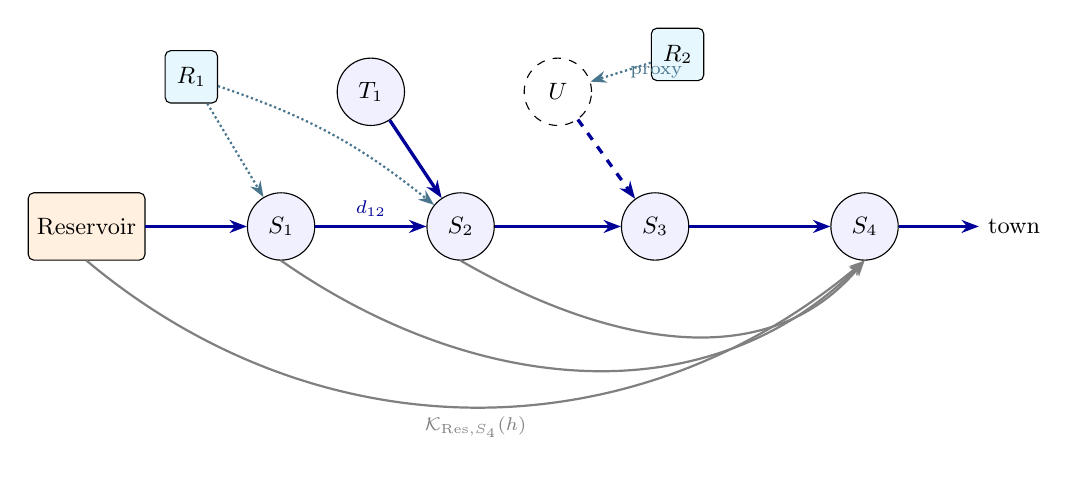
\begin{tikzpicture}[
  font=\small, scale=0.95, transform shape,
  st/.style={draw, circle, minimum size=9mm, fill=blue!6},
  rg/.style={draw, rounded corners=2pt, fill=cyan!10, minimum size=7mm},
  riv/.style={-{Stealth[length=2.2mm]}, very thick, blue!60!black},
  rainarr/.style={-{Stealth[length=2mm]}, densely dotted, thick, cyan!50!black},
  attn/.style={-{Stealth[length=2mm]}, gray, thick},
]
\node[draw, rounded corners=2pt, fill=orange!12, minimum height=9mm] (res) at (0,0) {Reservoir};
\node[st] (s1) at (2.6,0) {$S_1$};
\node[st] (s2) at (5.0,0) {$S_2$};
\node[st] (s3) at (7.6,0) {$S_3$};
\node[st] (s4) at (10.4,0) {$S_4$};
\node (town) at (12.4,0) {town};
\node[st] (t1) at (3.8,1.8) {$T_1$};
\node[draw, dashed, circle, minimum size=9mm] (u) at (6.3,1.8) {$U$};
\node[rg] (r1) at (1.4,2.0) {$R_1$};
\node[rg] (r2) at (7.9,2.3) {$R_2$};

\draw[riv] (res) -- (s1);
\draw[riv] (s1) -- node[above, font=\scriptsize] {$d_{12}$} (s2);
\draw[riv] (s2) -- (s3);
\draw[riv] (s3) -- (s4);
\draw[riv] (s4) -- (town);
\draw[riv] (t1) -- (s2);
\draw[riv, dashed] (u) -- (s3);
\draw[rainarr] (r1) -- (s1);
\draw[rainarr] (r1) to[bend left=10] (s2);
\draw[rainarr] (r2) -- node[right, font=\scriptsize] {proxy} (u);

\draw[attn] (res.south) to[out=-40, in=-140] node[below, font=\scriptsize] {$\K_{\Res,S_4}(h)$} (s4.south);
\draw[attn] (s1.south) to[out=-35, in=-135] (s4.south);
\draw[attn] (s2.south) to[out=-30, in=-130] (s4.south);
\end{tikzpicture}
\caption{River graph $\mathcal{G}$ (schematic). Blue: river flow. Dashed: the
unmonitored tributary $U$, represented in the model by the $R_2$ node (A5,
A11). Dotted: rain drainage. Grey: some of $S_4$'s attention edges. $S_4$
attends directly to all of
$\A(S_4)=\{\Res,S_1,S_2,S_3,T_1,R_1,R_2\}$, each restricted to its own lag
window.}
\label{fig:graph}
\end{figure}

% ===========================================================================
\section{Assumptions}
% ===========================================================================
\textbf{Supplied facts.}
\begin{enumerate}[label=\textbf{F\arabic*}, ref=F\arabic*, leftmargin=*]
  \item A forecast is issued every 10\,min, for the level 1\,h ahead at $S_1$--$S_4$.
  \item The reservoir releases upstream of $S_1$, and flow runs $S_1\!\to\!S_4$.
        The monitored tributary ($T_1$) joins between $S_1$ and $S_2$; the
        unmonitored one joins between $S_2$ and $S_3$.
  \item We have 10-minute level histories at $S_1$--$S_4$ and $T_1$; rainfall at
        $R_1$, $R_2$ with timestamps and locations; release records; and
        announced schedules with announcement and effective times.
  \item We have locations, connectivity and along-river distances. Spacing is
        uneven, and travel times vary.
  \item \emph{Not supplied:} travel times, or the unmonitored inflow.
        \emph{Not available at issuance:} future rainfall or future levels.
\end{enumerate}

\noindent\textbf{Assumptions} (statement; \emph{why}; \emph{effect on the design}).
\begin{enumerate}[label=\textbf{A\arabic*}, ref=A\arabic*, leftmargin=*]
  \item \textbf{Record length:} at least 3 years of overlapping data, including
  several floods. \emph{Why:} telemetry is normally archived.
  \emph{Effect:} about $1.5\times10^5$ issuance times, enough for a model of
  about $2\times10^5$ parameters.

  \item \textbf{Time base:} timestamps can be converted to UTC. Levels are
  instantaneous readings, and rain is the depth over the preceding 10\,min.
  Readings lie within $\pm5$\,min of the grid. \emph{Why:} this is standard for
  telemetry. \emph{Effect:} we align by snapping to the grid, with no temporal
  interpolation.

  \item \textbf{Delays:} most readings arrive within 5\,min, but outages can
  delay them by hours. Arrival times are logged. \emph{Why:} this is typical,
  and the brief does not specify delays. \emph{Effect:} features are built as of
  $t_0$, with an age channel and simulated delays (Section~\ref{sec:ops}).

  \item \textbf{Quality:} levels are accurate to $\pm2$\,cm, with spikes,
  flat-lines and up to 10\% gaps. Datums are fixed or documented.
  \emph{Why:} these are common sensor failure modes. \emph{Effect:} quality
  control turns bad readings into missing ones, every input carries a mask,
  and bad targets are excluded from the loss.

  \item \textbf{Rain gauges:} $R_1$ represents the slopes draining to the reach
  between the reservoir and $S_2$; $R_2$ represents the unmonitored
  tributary's catchment. \emph{Why:} these are the nearest gauges in the
  illustration. \emph{Effect:} this fixes the rain edges
  (Figure~\ref{fig:graph}). Attention learns how much each edge matters, so a
  wrong assignment degrades accuracy rather than breaking the model.

  \item \textbf{One-way influence:} levels are controlled from upstream, and
  backwater is negligible. \emph{Why:} it is a steep mountain river.
  \emph{Effect:} stations attend only to their ancestors (U8 covers the case
  where this fails).

  \item \textbf{Travel times:} wave celerity is $c\in[0.5,5]$\,m/s, so
  $\tau_{ji}\in[d_{ji}/c_{\max},\,d_{ji}/c_{\min}]$, and travel time shortens
  as flow rises. \emph{Why:} these are typical kinematic-wave
  speeds~\cite{chow}, widened because the true values are unknown.
  \emph{Effect:} physics fixes the lag-window bounds (Eq.~\ref{eq:window}),
  and the model learns the actual lag.

  \item \textbf{History window:} 24\,h covers the longest travel time, the rain
  response ($\le$12\,h) and one daily cycle. \emph{Why:} this can be checked
  against the supplied distances via
  $W\Delta=\max(24\,\mathrm{h},\tau^{\max}_{\Res,S_4}+6\,\mathrm{h})$.
  \emph{Effect:} $W=144$.

  \item \textbf{Releases:} records give the total outflow within 10\,min.
  Schedules are piecewise-constant, usually followed, but sometimes deviate.
  Past schedule versions are archived with their announcement times.
  \emph{Why:} this is standard gated-reservoir practice, and F3 states that
  announcement times exist. \emph{Effect:} a reservoir node with future steps;
  actual and scheduled channels; and training on the schedule as it was known.

  \item \textbf{$T_1$} lies near the confluence, so its level tracks the
  tributary's inflow. \emph{Effect:} $T_1$ is an ancestor of $S_2$--$S_4$,
  with a short lag window.

  \item \textbf{Unmonitored inflow} is a slow baseflow plus a response to rain
  over its catchment. \emph{Why:} rain is its only observable driver.
  \emph{Effect:} the $R_2$ node stands in for it, and $S_3$'s own history
  captures the baseflow.

  \item \textbf{Slow changes:} channel geometry, operating rules, snowmelt and
  evaporation change slowly compared with one hour and the retraining
  interval. \emph{Effect:} one model, retrained periodically, with calendar
  features and persistence covering the daily and seasonal cycles.

  \item \textbf{Target:} the target is the water level in metres above each
  station's datum. Alert levels $\theta_i$ are known; otherwise we use each
  station's 95th percentile. \emph{Effect:} no rating curve is needed, and the
  loss weights high water (Eq.~\ref{eq:loss}).

  \item \textbf{Infrastructure:} a server reads the telemetry in near real time
  and can publish within 2\,min. \emph{Effect:} the feasibility argument in
  Section~\ref{sec:ops}.
\end{enumerate}

% ===========================================================================
\section{Forecasting task and data specification}\label{sec:task}
% ===========================================================================
\textbf{Issuance time:} with $\Delta=10$\,min, a forecast is issued at every
grid time $t_0$ (UTC). $t_0$ is the data cut-off: only records \emph{received}
by $t_0$ are used. The forecast is published by $t_0+2$\,min.

\textbf{History window:} $k\in\{-143,\dots,0\}$, where step $k$ is time
$t_0+k\Delta$ (24\,h).

\textbf{Horizon:} $h\in\{1,\dots,6\}$, valid at $t_0+h\Delta$. The service
output is $h=6$ ($t_0+60$\,min). The other horizons add supervision.

\textbf{Outputs:} quantiles $q\in\mathcal{Q}=\{0.1,0.5,0.9\}$ of
$y_i(t_0+h\Delta)$ for $i\in\{S_1,\dots,S_4\}$.

\textbf{Batch:} one training sample is one issuance time, and $B$ indexes
them. In operation, $B=1$.

\begin{table}[H]
\centering\small
\caption{Model inputs and outputs.}
\label{tab:io}
\begin{tabularx}{\textwidth}{@{}l l L L@{}}
\toprule
\textbf{Tensor} & \textbf{Shape} & \textbf{Axes and content} & \textbf{Time coverage} \\
\midrule
$\mathbf{X}^{\mathrm{lev}}$ & $B\times144\times5\times3$ &
batch, step $k$, gauge ($S_1..S_4,T_1$), feature (level, forward-filled; mask $m$; age $a$) &
$(t_0-24\,\mathrm{h},\,t_0]$; records received by $t_0$ \\
$\mathbf{X}^{\mathrm{rain}}$ & $B\times144\times2\times3$ &
batch, step, gauge ($R_1,R_2$), feature (10-min depth; mask; age) &
step $k$ covers $(t_0+(k-1)\Delta,\,t_0+k\Delta]$ \\
$\mathbf{X}^{\mathrm{rel}}$ & $B\times144\times1\times4$ &
batch, step, reservoir, feature (recorded release; release scheduled for that step; record mask; minutes since announcement) &
$k=-143..0$; mean over each step \\
$\mathbf{F}^{\mathrm{rel}}$ & $B\times6\times1\times4$ &
the same features for future steps; the record slot holds the schedule, with mask 0 &
$(t_0,\,t_0+60\,\mathrm{min}]$; versions with $a\le t_0$ \\
$\mathbf{X}^{\mathrm{cal}}$ & $B\times150\times4$ &
batch, step, $\sin/\cos$ of time of day and day of year &
$k=-143..6$ \\
$\mathcal{G}$ & $23\times3$ &
edge $j\!\to\!i$ (ancestors and self-loops), ($d_{ji},\tau^{\min}_{ji},\tau^{\max}_{ji}$) &
static \\
$\bm{\ell}$ & $B\times4$ & batch, station: last valid level & latest valid reading by $t_0$ \\
\midrule
$\hat{\mathbf{Y}}$ (output) & $B\times4\times6\times3$ &
batch, station, horizon $h$, quantile &
$t_0+h\Delta$; served: $h=6$ \\
$\mathbf{Y},\mathbf{M}^{Y}$ & $B\times4\times6$ & observed future levels and their QC mask (training only) & $t_0+10..60$\,min \\
\bottomrule
\end{tabularx}
\end{table}

\textbf{Alignment across sampling times:} all series are mapped to one
10-minute UTC grid.
\begin{itemize}
  \item \textbf{Levels:} the latest valid reading within $\pm5$\,min of each
        grid time; otherwise the slot is marked missing.
  \item \textbf{Rain:} summed into the slot that ends at each grid time.
  \item \textbf{Releases:} averaged over each slot.
  \item \textbf{Schedules:} indexed by effective time $e$, and filtered by
        announcement time $a\le t_0$.
\end{itemize}

\textbf{Alignment across locations:} we do not interpolate in space. Each
source keeps its own token sequence as a node of $\mathcal{G}$, and the
distances become lag-window bounds and edge features. A type-specific
projection maps the different units and feature counts to width $d$.

\textbf{Available at issuance:} records received by $t_0$, and schedules
announced by $t_0$ (including those effective in $(t_0,t_0+60]$).
\textbf{Not available:} future levels and rain; actual future releases;
schedule changes announced after $t_0$; the unmonitored inflow; and readings
delayed past $t_0$.

% ===========================================================================
\section{Model computations and design justification}\label{sec:model}
% ===========================================================================
\textbf{Notation.} Nodes are
$\mathcal{V}=\{\Res,R_1,R_2,T_1,S_1,S_2,S_3,S_4\}$, and
$\mathcal{S}=\{S_1,\dots,S_4\}$ are the stations. $\A(i)$ is the set of nodes
whose water or rain reaches station $i$ (A5, A6):
$\A(S_1)=\{\Res,R_1\}$, $\A(S_2)=\A(S_1)\cup\{S_1,T_1\}$,
$\A(S_3)=\A(S_2)\cup\{S_2,R_2\}$, $\A(S_4)=\A(S_3)\cup\{S_3\}$.
$\mathbf{x}_{j,k}$ is node $j$'s feature vector at step $k$
(Table~\ref{tab:io}). Observed nodes have $k\le0$; the reservoir also has
$k=1..6$, from its schedule. $\mathbf{e}_j$, $\mathbf{e}^{\mathrm{cal}}_k$ and
$\mathbf{e}_h$ are learned node, calendar and horizon embeddings.

\paragraph{(1) Projection and temporal encoder.} Each node's inputs are
projected to width $d$ and passed through a causal dilated TCN~\cite{tcn},
whose weights are shared across nodes. With
$\mathbf{h}^{(0)}_{j,k}=\mathbf{u}_{j,k}$ and dilation $\delta_l=2^{l-1}$:
\begin{equation}
\begin{aligned}
  \mathbf{u}_{j,k} &= W^{\mathrm{in}}_{\mathrm{type}(j)}\mathbf{x}_{j,k} + \mathbf{e}_j + \mathbf{e}^{\mathrm{cal}}_k,\\
  \mathbf{h}^{(l)}_{j,k} &= \mathbf{h}^{(l-1)}_{j,k}
  + W^{(l)}_{o}\,\mathrm{GELU}\Big(\mathrm{LN}\Big(\textstyle\sum_{m=0}^{2}
     W^{(l)}_{m}\mathbf{h}^{(l-1)}_{j,\,k-m\delta_l}\Big)\Big),\quad l=1..7.
\end{aligned}
  \label{eq:tcn}
\end{equation}
Here $\mathbf{H}_{j,k}=\mathbf{h}^{(7)}_{j,k}$, and
$\mathbf{z}_i=\mathbf{H}_{i,0}$ is station $i$'s latest state. Earlier steps
are zero-padded. The receptive field is 255 steps, which covers the window,
and every output depends only on steps $\le k$.

\paragraph{(2) Physically bounded lag windows.} Water that reaches $i$ at
$t_0+h\Delta$ passed $j$ about $\tau_{ji}$ earlier. Using the bounds from A7,
the allowed steps of $j$ for forecast $(i,h)$ are
\begin{equation}
  \K_{ji}(h)=\big\{k:\ h-\lceil\tau^{\max}_{ji}/\Delta\rceil-\kappa \le k \le h-\lfloor\tau^{\min}_{ji}/\Delta\rfloor\big\}\cap\{k\le k^{\max}_j\}.
  \label{eq:window}
\end{equation}
\begin{itemize}
  \item $\kappa=3$ is a margin for attenuation of the wave.
  \item $k^{\max}_j=0$ for observed nodes; $k^{\max}_{\Res}=6$, because the
        schedule is known.
  \item An empty window becomes $\{0\}$: the model extrapolates from the latest
        state.
  \item River edges use $\tau^{\min}=d/c_{\max}$ and $\tau^{\max}=d/c_{\min}$;
        rain edges use $[0,12\,\mathrm{h}]$; self-edges use the last 2\,h.
\end{itemize}
\emph{Example:} with $d_{12}=6$\,km, $\tau_{12}\in[20,200]$\,min, so
$\K_{S_1S_2}(6)=\{-17,\dots,0\}$. The upper bound ($k\le4$) is cut at 0,
because some water that reaches $S_2$ within the hour has not yet passed $S_1$.
This is a physical limit that no model can remove (U2).

\paragraph{(3) Directed lag-attention~\cite{transformer}.} For station $i$ and
horizon $h$, the candidate tokens are
$\mathcal{T}_i(h)=\{(j,k):j\in\A(i)\cup\{i\},\,k\in\K_{ji}(h)\}$. For each head
$r=1..4$:
\begin{equation}
\begin{aligned}
  \alpha^{(r)}_{i,h}(j,k)&=\operatorname*{softmax}_{(j,k)\in\mathcal{T}_i(h)}
   \frac{\big(W^{(r)}_Q[\mathbf{z}_i\|\mathbf{e}_h]\big)^{\!\top} W^{(r)}_K\mathbf{c}_{j,k}}{\sqrt{d/4}},\\
  \mathbf{m}_{i,h}&=W_O\Big\Vert_{r=1}^{4}\sum_{(j,k)\in\mathcal{T}_i(h)}\alpha^{(r)}_{i,h}(j,k)\,W^{(r)}_V\mathbf{c}_{j,k},
\end{aligned}
  \label{eq:attn}
\end{equation}
where $\mathbf{c}_{j,k}=[\mathbf{H}_{j,k}\,\|\,\psi(h-k,d_{ji},j)]$, and $\psi$
is an MLP that encodes the lag, the distance and the source type. Tokens
outside $\mathcal{T}_i(h)$ get zero weight; this is where the physics enters
as a hard constraint.

\paragraph{(4) Forecast mapping.} The decoder computes
$(\delta,a,b)_{i,h}=\mathrm{MLP}([\mathbf{z}_i\|\mathbf{m}_{i,h}\|\mathbf{e}_i\|\mathbf{e}_h])$,
anchored on the last valid level $\ell_i$:
\begin{equation}
  \hat y^{0.5}_{i,h}=\ell_i+\sigma_i\delta_{i,h},\quad
  \hat y^{0.1}_{i,h}=\hat y^{0.5}_{i,h}-\sigma_i\,\mathrm{softplus}(a_{i,h}),\quad
  \hat y^{0.9}_{i,h}=\hat y^{0.5}_{i,h}+\sigma_i\,\mathrm{softplus}(b_{i,h}),
  \label{eq:out}
\end{equation}
Here $\sigma_i$ is the standard deviation of station $i$'s 1-hour level change.
The softplus terms make the quantiles non-crossing. Together,
Eqs.~(\ref{eq:tcn})--(\ref{eq:out}) define the forecast mapping
$\hat{\mathbf{Y}}=f_\theta(\mathbf{X}^{\mathrm{lev}},\mathbf{X}^{\mathrm{rain}},\mathbf{X}^{\mathrm{rel}},\mathbf{F}^{\mathrm{rel}},\mathbf{X}^{\mathrm{cal}};\mathcal{G})$.

\paragraph{(5) Training objective.} A masked pinball loss~\cite{koenker}, with
$\rho_q(e)=\max(qe,(q-1)e)$:
\begin{equation}
  \mathcal{L}(\theta)=\frac{1}{\sum M^{Y}}\sum_{b,i,h}M^{Y}_{b,i,h}\,w_h\,\omega_{b,i,h}
  \sum_{q\in\mathcal{Q}}\rho_q\Big(\frac{y_{b,i,h}-\hat y^{q}_{b,i,h}}{\sigma_i}\Big)+\lambda\|\theta\|^2,
  \label{eq:loss}
\end{equation}
\begin{itemize}
  \item $w_6=2$ and $w_{h<6}=1$, so the served horizon counts most.
  \item $\omega=1+4\cdot\mathbf{1}[y>\theta_i]$ gives extra weight to floods
        (A13).
  \item \textbf{Protocol:} chronological train/validation/test split by year;
        Adam with early stopping on the validation loss at $h=6$; masking and
        delay augmentation; a 5-seed ensemble.
  \item \textbf{Size:} about $1.9\times10^5$ parameters.
  \item \textbf{Deployment test:} the model must beat persistence and
        schedule-aware linear routing at $h=6$, especially on floods.
\end{itemize}

\begin{table}[H]
\centering\small
\caption{How each driver reaches the forecasts.}
\label{tab:drivers}
\begin{tabularx}{\textwidth}{@{}l L l@{}}
\toprule
\textbf{Driver} & \textbf{Path in the model} & \textbf{Affects} \\
\midrule
Upstream levels & tokens of upstream $S_j$ in $\K_{ji}(h)$; the weight peaks at the current travel time & $S_2$--$S_4$ \\
Monitored tributary & $T_1$ tokens, with a short window (A10) & $S_2$--$S_4$ \\
Unmonitored tributary & $R_2$ tokens (its catchment's rain), plus $S_3$'s own history (baseflow) & $S_3,S_4$ \\
Rainfall & past $R_1/R_2$ tokens within the response window; future rain is unknown & $R_1$: all; $R_2$: $S_3,S_4$ \\
Reservoir & recorded releases ($k\le0$) and the announced schedule ($k=1..6$), at distance-based lags & all; fastest at $S_1$ \\
Own state & self-tokens (last 2\,h) and the anchor $\ell_i$ & each \\
\bottomrule
\end{tabularx}
\end{table}

\textbf{Physical assumptions and learned mappings.} \emph{Imposed by physics:}
flow direction (A6); which sources can affect which station (F2, A5);
causality, with only announced schedules as future inputs; travel-time bounds
(A7); and the persistence anchor. \emph{Learned:} the actual lag within each
window and its dependence on flow (through $\mathbf{z}_i$ and
$\mathbf{H}_{j,k}$); attenuation of the wave; the rainfall--runoff response;
tributary contributions, including the unmonitored one; nonlinear
relationships between stations; and the width of the uncertainty.
We use no separate simulator: physics enters as structure, not as equations to
solve. This stays robust when travel times and inflows are unknown.

\textbf{Justification.}
\begin{enumerate}[label=\textbf{J\arabic*}, ref=J\arabic*, leftmargin=*]
  \item \textbf{Spatial input is necessary.} In the companion notebook,
  temporal-only models give one forecast for identical local histories. That
  forecast is the mean (MSE) or median (MAE) of the possible outcomes. An
  upstream rise that has not yet arrived is exactly such a case.

  \item \textbf{Keep timing.} Telling which node saw a rise first needs one
  vector per time step (Think about 2), so the TCN does not pool over time.

  \item \textbf{Reach.} One local S--T pair or ST block reaches 1 node and 2
  steps (Think about 3). The reservoir is 4 hops and tens of steps from $S_4$.
  Direct ancestor edges with attention give full reach in one layer, as
  attention did over a 3-block ST stack in the relay experiment (Think about 4).

  \item \textbf{Mask the attention.} Full attention over $L=1200$ tokens costs
  $2L^2d\approx1.8\times10^8$ operations, which is affordable. But it allows
  physically impossible dependencies, which are a real risk with few floods
  (A1). Masking keeps the reach and encodes what we know.

  \item \textbf{Direct multi-horizon outputs and a persistence anchor.} There is
  no error accumulation from autoregressive feedback, and the announced future
  enters naturally, as in TFT~\cite{tft}. The model's capacity goes to events
  rather than to steady periods.

  \item \textbf{Quantiles.} Under missing information, MSE returns a mean that
  may be implausible (Think about 1). Quantiles give the median and a
  calibrated range, which is what flood preparedness needs.

  \item \textbf{Alternatives.} A per-station LSTM cannot see upstream.
  Neighbour-only GNNs (DCRNN~\cite{dcrnn}, Graph WaveNet~\cite{gwn}) need
  several hops. Pure Muskingum routing~\cite{chow} needs travel times and
  inflows we do not have. Our design follows data-driven rainfall--runoff
  models~\cite{kratzert}, with a river graph added.
\end{enumerate}

% ===========================================================================
\section{Operation and exceptional conditions}\label{sec:ops}
% ===========================================================================
\textbf{(i) Missing observations.}
\begin{itemize}
  \item Quality control (A4) marks gaps, out-of-range values, spikes and
        flat-lines as missing.
  \item A missing input is forward-filled, with mask $m=0$ and a growing age
        $a$, so the model knows a reading is stale and by how much.
  \item Training randomly masks 5--20\% of readings, and sometimes whole sensors
        for 1--12\,h. The model therefore learns other paths: for example, if
        $S_2$ is down, $S_3$ leans on $S_1$ and $T_1$ at longer lags.
  \item Missing targets are excluded from the loss.
  \item If a station's own sensor is missing, its anchor is the last valid
        value, its range widens, and the forecast is flagged \emph{degraded}.
  \item After more than 6\,h without data, or if all ancestors are missing, the
        station falls back to persistence plus schedule-aware routing,
        flagged \emph{fallback}.
\end{itemize}

\textbf{(ii) Delayed observations.}
\begin{itemize}
  \item Each record stores its observation time and its arrival time.
  \item Features use an as-of join (arrival $\le t_0$), so a late reading looks
        like a missing reading with growing age. Training simulates delays
        drawn from the logged distribution (A3), so it sees the same
        situation.
  \item The forecast never waits for data.
  \item Late data enters the next issuance, 10\,min later. If it moves the
        60-minute median by more than 5\,cm, an updated forecast is issued
        immediately.
  \item Each forecast's inputs are logged for audit.
\end{itemize}

\textbf{(iii) Announced future releases.}
\begin{itemize}
  \item The reservoir's steps $k=1..6$ come from the latest schedule with
        $a\le t_0$.
  \item Releases effective after $t_0+60$\,min cannot affect the hour, so they
        are excluded.
  \item The lag windows send a release effective at $e$ to station $i$ near
        $e+\tau_{\Res,i}$. A change at $t_0+20$\,min therefore lifts the $S_1$
        forecast only for $t_0+30..60$.
  \item ``Minutes since announcement'' lets the model learn that last-minute
        schedules are less reliable.
  \item Training uses each schedule \emph{as it was known} at $t_0$ (A9), never
        the outcome, so there is no leakage.
\end{itemize}

\textbf{(iv) Scheduled versus actual releases.}
\begin{itemize}
  \item Past reservoir tokens hold both the \emph{recorded} release and the
        release \emph{scheduled} for that step; future tokens hold only the
        schedule.
  \item The model therefore learns typical deviations, such as a late start,
        and the quantiles absorb the rest.
  \item \textbf{Live detection:} $S_1$ sits just below the dam, so a deviation
        appears there first. If the record, or $S_1$'s response, departs from
        the schedule beyond a threshold, the next issuance uses the record, the
        forecast is flagged \emph{schedule deviation}, and the operator is
        asked to confirm.
  \item A missing record is replaced by the schedule, with $m=0$.
  \item An emergency release enters the next issuance as a new schedule version.
\end{itemize}

\textbf{Feasibility.} One issuance ($B=1$, 1200 tokens, $d=64$) costs about
$7\times1200\times4d^2\approx1.4\times10^8$ multiply-adds in the TCN, plus
about $10^7$ for 24 attention queries. That is under 0.3\,GFLOP, or 10--50\,ms
on one CPU core, and the 5-member ensemble stays under 1\,s. Building the
features reads about 1200 values. The full cycle (fetch, quality control,
inference, publish, log) fits easily within 2 minutes. Retraining
($\sim\!1.5\times10^5$ samples) takes minutes on one GPU, run monthly or on
drift. A watchdog restarts failed runs, and the persistence fallback is
published if the model is unavailable.

% ===========================================================================
\section{Uncertainty, limitations, and additional information}\label{sec:unc}
% ===========================================================================
Each item gives its impact, our response, and what remains unresolved.
\begin{enumerate}[label=\textbf{U\arabic*}, ref=U\arabic*, leftmargin=*]
  \item \textbf{Unmonitored tributary.} \emph{Impact:} storms over its
  catchment raise $S_3$ and $S_4$ with no upstream warning, so the median
  lags. \emph{Response:} the $R_2$ proxy, $S_3$'s own trend, and wider
  $S_3$/$S_4$ ranges when $R_2$ is wet. \emph{Unresolved:} storms that $R_2$
  misses (D3).

  \item \textbf{Changing travel times.} \emph{Impact:} a fixed lag mistimes
  peaks. \emph{Response:} attention picks the lag from the current state,
  within wide bounds. We check the learned lags against physics on recorded
  events. \emph{Unresolved:} overbank floods may fall outside the bounds
  (D4). On short reaches, water arriving within the hour is partly
  unobserved (Eq.~\ref{eq:window}).

  \item \textbf{Future rain.} \emph{Impact:} rain after $t_0$ on fast slopes
  causes under-prediction. \emph{Response:} ranges that reflect recent rain.
  \emph{Unresolved} without D5.

  \item \textbf{Rare extremes.} \emph{Impact:} networks extrapolate poorly.
  \emph{Response:} the anchor, flood weighting, an ``outside training range''
  flag, and the routing fallback. \emph{Unresolved:} unprecedented floods,
  where forecasts are indicative only.

  \item \textbf{Sparse rain gauges.} \emph{Impact:} two gauges miss rain that
  varies over mountains. \emph{Response:} learned weights and wider ranges
  (D5, D6).

  \item \textbf{Sensor drift and datum shifts.} \emph{Response:} quality
  control, checks against neighbouring stations, and maintenance logs (D1).
  \emph{Unresolved:} slow drift can look like real change.

  \item \textbf{Non-stationarity} (sediment, vegetation, new rules).
  \emph{Response:} monitor rolling error and coverage; retrain monthly or on
  drift (A12).

  \item \textbf{Backwater} at high tributary flows violates A6.
  \emph{Response:} add a downstream edge if validation errors show it.

  \item \textbf{Calibration under shift.} \emph{Response:} conformalised
  quantile recalibration~\cite{cqr} on a rolling window keeps 80\% coverage;
  the ensemble spread adds epistemic uncertainty.

  \item \textbf{Release deviations.} \emph{Response:} Section~\ref{sec:ops}(iv),
  plus telemetry (D2).
\end{enumerate}

\noindent\textbf{Additional information requests.} The system works with the
supplied data alone; each request improves it.

\begin{table}[H]
\centering\small
\caption{Additional information requested.}
\label{tab:requests}
\begin{tabularx}{\textwidth}{@{}l L L l@{}}
\toprule
\textbf{ID} & \textbf{Request} & \textbf{How it helps} & \textbf{Usable without?} \\
\midrule
D1 & Record length, latency logs, QC and maintenance metadata & Confirms A1--A4; realistic delay simulation & Yes (assumed) \\
D2 & Archived schedule versions; gate and spillway telemetry & Training without leakage; early deviation detection & Yes, wider ranges \\
D3 & A gauge, even a temporary one, on the unmonitored tributary & Observes the main unknown; added as a new node, no redesign & Yes, wider $S_3/S_4$ \\
D4 & Cross-sections, travel-time studies, or a hydraulic model & Tighter $[\tau^{\min},\tau^{\max}]$; validates lags; a better fallback & Yes, wide bounds \\
D5 & Radar or rainfall nowcasts for the next hour & Future rain, as a known-future input (U3) & Yes, lower skill \\
D6 & More rain gauges; snow and temperature data & Spatial rain coverage; snowmelt & Yes \\
D7 & Rating curves and discharge data & Mass-balance checks; discharge extension & Yes \\
D8 & Official alert levels and how forecasts are used & Sets $\theta_i$ and which quantile to act on & Yes (95th pct.) \\
\bottomrule
\end{tabularx}
\end{table}

% ===========================================================================
{\small
\begin{thebibliography}{9}\setlength{\itemsep}{0pt}
\bibitem{tcn} S.~Bai, J.~Z. Kolter, V.~Koltun. An empirical evaluation of generic convolutional and recurrent networks for sequence modeling. \emph{arXiv:1803.01271}, 2018.
\bibitem{transformer} A.~Vaswani et al. Attention is all you need. \emph{NeurIPS}, 2017.
\bibitem{koenker} R.~Koenker, G.~Bassett. Regression quantiles. \emph{Econometrica} 46(1), 1978.
\bibitem{tft} B.~Lim, S.~\"O. Ar{\i}k, N.~Loeff, T.~Pfister. Temporal Fusion Transformers for interpretable multi-horizon time series forecasting. \emph{Int.\ J.\ Forecasting} 37(4), 2021.
\bibitem{dcrnn} Y.~Li, R.~Yu, C.~Shahabi, Y.~Liu. Diffusion convolutional recurrent neural network: data-driven traffic forecasting. \emph{ICLR}, 2018.
\bibitem{gwn} Z.~Wu, S.~Pan, G.~Long, J.~Jiang, C.~Zhang. Graph WaveNet for deep spatial-temporal graph modeling. \emph{IJCAI}, 2019.
\bibitem{kratzert} F.~Kratzert et al. Rainfall--runoff modelling using Long Short-Term Memory (LSTM) networks. \emph{Hydrology and Earth System Sciences} 22, 2018.
\bibitem{chow} V.~T. Chow, D.~R. Maidment, L.~W. Mays. \emph{Applied Hydrology}. McGraw-Hill, 1988.
\bibitem{cqr} Y.~Romano, E.~Patterson, E.~Cand\`es. Conformalized quantile regression. \emph{NeurIPS}, 2019.
\end{thebibliography}

% ===========================================================================
\section*{Generative AI usage disclosure}
% ===========================================================================
\textbf{Tool:} Claude (Anthropic), used through Claude Code.

\noindent\textbf{Prompts} (verbatim, in order):
(1)~``this is the assignment document, that explains what the problem statement is, what is required to do and what is already provided. Please read this doc thoroughly and explain to me..''
(2)~``lets start with question 1. please explain how will we solve it ?''
(3)~``so you're saying, I need to run Question1/Question1.ipynb . Do I need to odify anything in that or is it good to run?''
(4)~``to run that notebook on google colab, what do i need to do ?''
(5)~``let me run it on my mac then''
(6)~``why did it open a localhost ?''
(7)~``so I run the notebook. Was ZI supposed to change anything ?''
(8)~``tell me step by step what i need to do''
(9)~``how do test the four prompts?''
(10)~``for each prompt, what do I need to do in the notebook ?''
(11)~``You have to write me complete report for question 1. Tell me what you need from me?''
(12)~``name: Muhammad Sikander Raheem, roll Number: 25280017, no github repolink yet. please use latex/overleaf. For architecture use defaults. Please write the report and I'll compile it in overleaf''
(13)~``This is a 12 page report. Can you please make it 7-9 pages''

\noindent\textbf{Outputs:}
\begin{itemize}
  \item an explanation of the assignment;
  \item a solution approach for Question 1;
  \item instructions for running the notebook;
  \item worked reasoning for its ``Think about'' prompts;
  \item a full LaTeX draft of this report (architecture, assumptions, equations,
        operations, limitations, TikZ figures), then a condensed version.
\end{itemize}

\noindent\textbf{Edits made by the student:}
\todo{describe what you changed, checked, or rewrote}
}
\end{document}
